\documentclass[conference]{IEEEtran}
\IEEEoverridecommandlockouts

\usepackage[spanish,es-tabla,es-noshorthands]{babel}
\usepackage{amsmath,amssymb}
\usepackage{graphicx}
\usepackage{booktabs}
\usepackage{array}
\usepackage{url}
\usepackage{cite}

\AtBeginDocument{%
  \renewcommand{\tablename}{Tabla}%
  \renewcommand{\figurename}{Fig.}%
}

\begin{document}

\title{Selección de atributos mediante optimización por enjambre de partículas binaria para la predicción de calidad del vino con Random Forest}

\author{%
\IEEEauthorblockN{Ivan Renée Paredes Ozuna}
\IEEEauthorblockA{\textit{Facultad Politécnica}\\
\textit{Universidad Nacional de Asunción}\\
San Lorenzo, Paraguay}
\and
\IEEEauthorblockN{Sergio Ramon Gonzalez Silva}
\IEEEauthorblockA{\textit{Facultad Politécnica}\\
\textit{Universidad Nacional de Asunción}\\
San Lorenzo, Paraguay}
\thanks{Trabajo práctico final del Grupo~5, asignatura Machine Learning, Facultad Politécnica, Universidad Nacional de Asunción (FP-UNA).}%
}

\maketitle

\begin{abstract}
La calidad sensorial del vino se estima habitualmente mediante cata, un procedimiento costoso y variable. Este trabajo examina si la optimización por enjambre de partículas binaria permite reducir las once variables fisicoquímicas del conjunto Wine Quality (vinos tintos, repositorio UCI, 1599 muestras) sin degradar un clasificador Random Forest. La puntuación original se transforma en una etiqueta binaria con el umbral \emph{quality} $\geq 6$. Se reserva un 20\,\% estratificado para prueba y la búsqueda se ejecuta solo sobre desarrollo, con validación cruzada estratificada de tres particiones. La función objetivo minimiza uno menos el F1-macro de validación más una penalización proporcional al número de atributos. Con 30 evaluaciones por ejecución y cinco semillas, la solución de menor costo retiene cinco atributos. Su F1-macro de validación es 0,787, frente a 0,783 del modelo con las once variables. En la prueba, evaluada una sola vez, el F1-macro pasa de 0,786 a 0,764. Alcohol y sulfatos aparecen en las cinco ejecuciones, pero los subconjuntos no son estables y la trayectoria seleccionada no mejora después de la primera evaluación. Bajo este presupuesto, la búsqueda simplifica el modelo a costa de una pérdida predictiva que no se compensa en el conjunto reservado.
\end{abstract}

\begin{IEEEkeywords}
calidad del vino, selección de atributos, Random Forest, enjambre de partículas binario, validación cruzada
\end{IEEEkeywords}

\section{Introducción}
La calidad comercial del vino se decide, en gran medida, por una evaluación sensorial. Esa medición es útil, pero depende de catadores, no se obtiene en el mismo momento que el análisis de laboratorio y resulta difícil de repetir a escala. Los atributos fisicoquímicos ---acidez, anhídrido sulfuroso, densidad, pH, sulfatos o grado alcohólico--- sí pueden medirse de forma rutinaria. El conjunto Wine Quality mostró que esas variables contienen información sobre la preferencia sensorial y, al mismo tiempo, dejó abierta la pregunta de si todas ellas son necesarias~\cite{cortez2009}.

Usar las once variables no es gratuito. Algunas pueden ser redundantes, otras pueden aportar poco a la frontera de decisión y el modelo resultante es más difícil de interpretar en términos de proceso enológico. La selección de atributos busca un subconjunto pequeño que conserve el desempeño~\cite{guyon2003,kohavi1997}. Cuando el criterio depende del clasificador, el enfoque natural es un método \emph{wrapper}: cada candidato se valora entrenando el modelo que luego se va a utilizar.

El espacio de este problema tiene $2^{11}=2048$ subconjuntos. Es finito, pero evaluarlo de forma exhaustiva con un ensamble y validación cruzada sigue siendo más costoso de lo que el presupuesto experimental permite. Las metaheurísticas ofrecen una exploración parcial guiada por el valor de la función objetivo. La optimización por enjambre de partículas (PSO) actualiza un conjunto de soluciones a partir de la memoria individual y de la memoria de la vecindad~\cite{kennedy1995}. Su variante binaria representa precisamente la decisión de incluir o excluir cada atributo~\cite{kennedy1997}.

El clasificador de referencia es Random Forest~\cite{breiman2001}. Se mantiene con hiperparámetros fijos para que la comparación aísle el efecto de la selección y no se confunda con un ajuste del ensamble. El objetivo es determinar si el enjambre binario obtiene un bosque más parsimonioso que mantenga, o no, el rendimiento predictivo del modelo con las once variables.

Las contribuciones de este trabajo son experimentales y no consisten en un algoritmo nuevo. Se formula un costo que equilibra el F1-macro de validación y el número de atributos; se fija un protocolo con prueba reservada, tres particiones estratificadas y cinco semillas; y se documentan la convergencia, la estabilidad y el tiempo de búsqueda con los resultados obtenidos. El resto del artículo revisa los fundamentos, describe materiales y métodos, discute los resultados y cierra con las limitaciones que esos resultados imponen.

\section{Fundamentos y trabajos relacionados}

\subsection{Random Forest}
Random Forest construye varios árboles sobre muestras \emph{bootstrap} y, en cada división, considera un subconjunto aleatorio de atributos~\cite{breiman2001}. El voto de los árboles reduce la varianza de un único árbol y se comporta bien en tablas de tamaño moderado, con relaciones no lineales y con valores extremos. En clasificación, la predicción es la clase mayoritaria y las probabilidades estimadas permiten calcular el área bajo la curva ROC.

El propio ensamble ya realiza una forma interna de selección en cada nodo. Esa selección local no responde, sin embargo, a la pregunta de cuáles variables deben entrar al modelo final. Un \emph{wrapper} externo responde otra pregunta: qué subconjunto, evaluado de extremo a extremo, sostiene el desempeño del bosque completo. Por eso los hiperparámetros del bosque se dejan fijos. Si se optimizaran junto con la máscara, no sería posible atribuir un cambio de métrica a la selección de atributos.

\subsection{Optimización por enjambre de partículas}
En PSO, cada partícula es una solución candidata. Su velocidad se corrige con un término de inercia, un término cognitivo hacia la mejor posición visitada por la partícula y un término social hacia la mejor posición de su vecindario~\cite{kennedy1995}. La variante binaria no actualiza la posición de forma continua. PySwarms, la biblioteca utilizada, aplica la regla documentada por Kennedy y Eberhart~\cite{kennedy1997,miranda2018}: la velocidad sigue el esquema continuo y la coordenada binaria se obtiene al comparar un número aleatorio con una sigmoide de esa velocidad. La topología implementada es un anillo de mejor local, no un mejor global único.

Esa distinción importa para leer los resultados. Con pocos vecinos y pocas iteraciones, el enjambre puede quedar cerca de la inicialización. Un buen costo observado en la primera evaluación no demuestra que la dinámica de búsqueda haya encontrado esa solución.

\subsection{Selección de atributos}
La selección de variables persigue tres efectos: reducir dimensión, disminuir el efecto de atributos irrelevantes y hacer más interpretable el predictor~\cite{guyon2003}. Los métodos de filtro ordenan variables con una medida independiente del clasificador. Los \emph{wrapper} usan el error del propio modelo y, por eso, capturan interacciones que una correlación marginal no ve~\cite{kohavi1997}. El costo es el número de entrenamientos.

El compromiso entre desempeño y tamaño del subconjunto puede plantearse como un único objetivo penalizado o como un frente de Pareto. Xue, Zhang y Browne mostraron que un PSO multiobjetivo puede devolver varios subconjuntos no dominados y que la selección evolutiva compite con filtros clásicos~\cite{xue2013,xue2016}. El presente experimento es más restringido: un solo objetivo, un clasificador fijo, un presupuesto de 30 evaluaciones por ejecución y un único conjunto de datos. No se pretende mejorar esos métodos; se los usa como marco para interpretar una penalización lineal pequeña.

\subsection{Predicción de calidad del vino}
Cortez \emph{et al.} ajustaron regresión y clasificación sobre las propiedades fisicoquímicas de vinos tintos y blancos de \emph{vinho verde} y compararon máquinas de vectores de soporte, redes neuronales y regresión múltiple~\cite{cortez2009}. El trabajo ya advertía que las clases están desbalanceadas y que no era evidente que todas las entradas fueran relevantes. Esa observación es el punto de partida de la selección estudiada aquí. No se reproducen sus modelos ni se comparan cifras de error con las de ese artículo, porque la etiqueta, la partición y la métrica no coinciden.

\section{Materiales y métodos}

\subsection{Conjunto de datos}
Se utiliza exclusivamente \texttt{winequality-red.csv} del repositorio UCI Machine Learning~\cite{cortez2009,uci186}. El archivo se descarga de la URL pública del repositorio, está separado por punto y coma y contiene 1599 registros, once atributos numéricos y la puntuación sensorial \emph{quality}, un entero observado entre 3 y 8. No se mezcla con el archivo de vinos blancos: las dos poblaciones no comparten la misma distribución fisicoquímica y el enunciado del trabajo fija once atributos. El conjunto es de uso académico, condicionado a citar a los autores originales. No se identificó un número de versión distinto de la publicación de 2009.

La Tabla~\ref{tab:dataset} resume la estructura. No hay valores faltantes. Hay 240 filas duplicadas exactas, el 15,0\,\% de la muestra. Se conservan: pueden corresponder a perfiles fisicoquímicos repetidos y eliminarlas alteraría la frecuencia de las puntuaciones. Tampoco se eliminan extremos. Random Forest admite colas pesadas y un valor atípico puede ser un vino informativo. En desarrollo, el criterio de Tukey marca sobre todo al azúcar residual (9,6\,\%) y a los cloruros (6,3\,\%).

\begin{table}[!t]
\caption{Caracterización del conjunto de vinos tintos}
\label{tab:dataset}
\centering
\footnotesize
\begin{tabular}{@{}ll@{}}
\toprule
Elemento & Valor observado \\
\midrule
Registros / atributos & 1599 / 11 \\
Variable objetivo & \emph{quality} $\in \{3,\ldots,8\}$ \\
Valores faltantes & 0 \\
Duplicados exactos & 240 (15,0\,\%) \\
Desarrollo / prueba & 1279 / 320 (80/20) \\
Clase alta en desarrollo & 684 (53,5\,\%) \\
Clase baja en desarrollo & 595 (46,5\,\%) \\
\bottomrule
\end{tabular}
\end{table}

La puntuación está concentrada en 5 y 6: 681 y 638 vinos, respectivamente. Las colas son escasas: 10 vinos de calidad 3, 53 de calidad 4, 199 de calidad 7 y 18 de calidad 8. Un clasificador multiclase de seis categorías dejaría particiones de validación con muy pocos ejemplos extremos. Por eso se adopta la etiqueta binaria
\begin{equation}
y =
\begin{cases}
1, & \text{si } \mathit{quality} \geq 6,\\
0, & \text{si } \mathit{quality} \leq 5,
\end{cases}
\label{eq:umbral}
\end{equation}
después de inspeccionar la distribución de desarrollo. El corte $\geq 6$ separa una calidad baja o media-baja de una calidad aceptable o alta y produce dos clases con soporte suficiente. En el conjunto completo quedan 855 vinos de clase alta (53,5\,\%) y 744 de clase baja (46,5\,\%). La limitación es clara: un vino de 6 y uno de 8 comparten etiqueta, de modo que el modelo no distingue excelencia de simple aceptabilidad.

\subsection{Análisis exploratorio y preprocesamiento}
El análisis descriptivo que condiciona decisiones se calcula sobre desarrollo. La Fig.~\ref{fig:quality} muestra la concentración en las puntuaciones centrales. La correlación de Spearman más alta con \emph{quality} corresponde al alcohol (0,489), seguida por la acidez volátil ($-0{,}376$) y los sulfatos (0,362). El azúcar residual es casi independiente de la puntuación (0,036).

Ningún par de atributos alcanza $|r|=0{,}70$ en desarrollo. Las asociaciones lineales más fuertes son acidez fija con pH ($-0{,}675$), con densidad (0,669) y con ácido cítrico (0,662), además de la relación entre anhídrido sulfuroso libre y total (0,658). Hay redundancia moderada, no un par sustituible de forma evidente. Esa es una razón adicional para preferir un \emph{wrapper} frente a descartar variables solo por correlación.

\begin{figure}[!t]
\centering
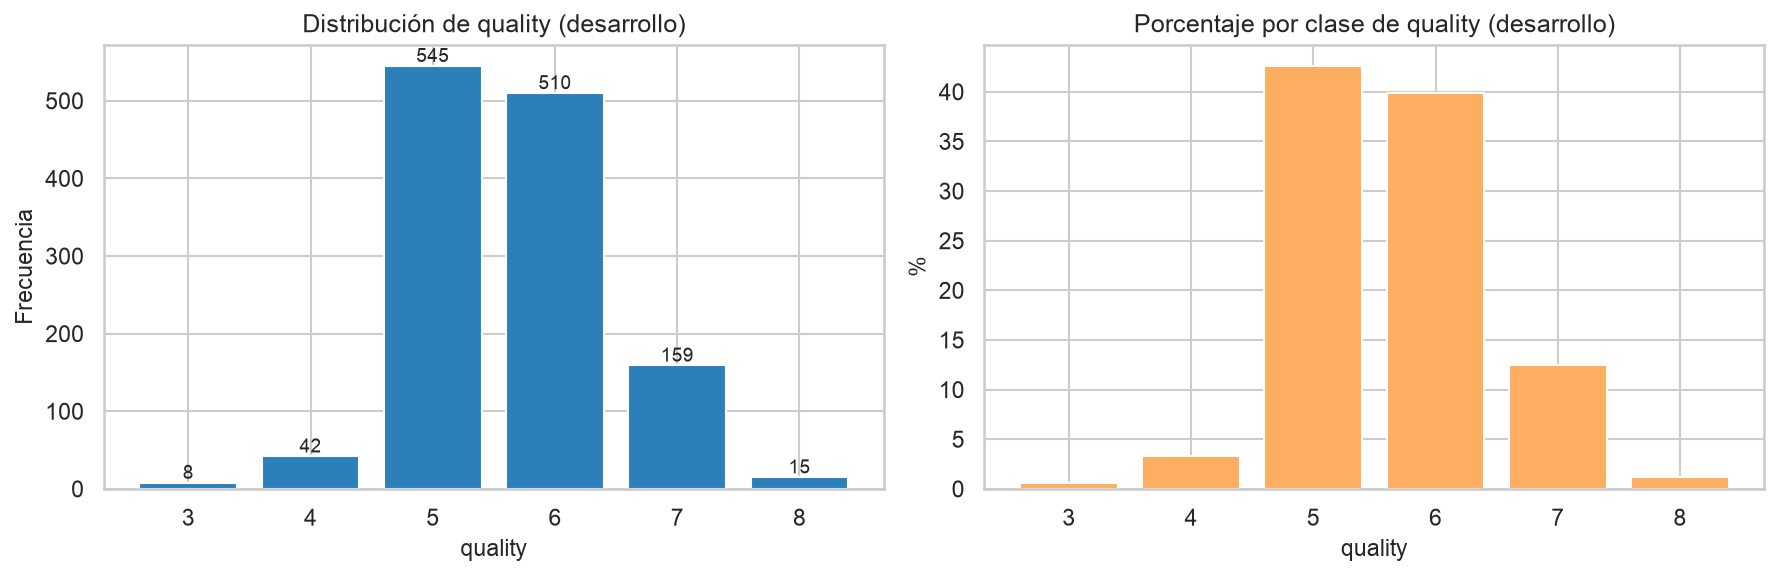
\includegraphics[width=\columnwidth]{figuras/distribucion_quality.png}
\caption{Distribución de \emph{quality} en el conjunto de desarrollo, antes de la binarización.}
\label{fig:quality}
\end{figure}

La partición se hace antes de binarizar y antes de la búsqueda. Con semilla 42 se separa el 20\,\% de prueba de forma estratificada sobre \emph{quality}. El 80\,\% restante es el único material de la validación y del enjambre. La prueba queda reservada hasta la evaluación final y no interviene en la máscara elegida. Dentro de desarrollo se usa validación cruzada estratificada de tres particiones, con barajado y semilla 42, la misma para todas las comparaciones. No hay imputación. El escalado se incluye en un \emph{pipeline} y se ajusta solo en el pliegue de entrenamiento de cada partición. Random Forest no lo requiere; se mantiene para que cualquier transformación quede dentro del protocolo y no se estime con la prueba.

\subsection{Modelo de referencia}
El bosque de referencia usa las once variables. Los hiperparámetros, idénticos en todas las comparaciones, son 100 árboles, profundidad máxima 12, mínimo de dos muestras por hoja y $\sqrt{p}$ atributos candidatos en cada división. La profundidad y el tamaño de hoja limitan el ajuste de un ensamble grande para 1279 filas; 100 árboles equilibran estabilidad y tiempo en CPU. No se realiza búsqueda de hiperparámetros, porque el factor experimental es la máscara de atributos.

La métrica principal es el F1-macro: el promedio no ponderado del F1 de cada clase. Se prefiere a la exactitud porque la clase alta es solo moderadamente mayoritaria y el F1-macro penaliza un fallo concentrado en una clase. Como métricas secundarias se registran la exactitud balanceada, la precisión y la sensibilidad macro, la exactitud y el AUC-ROC. Este último es válido porque el problema final es binario y el bosque entrega probabilidades.

En desarrollo, el modelo de once atributos obtiene un F1-macro de $0{,}783 \pm 0{,}013$, exactitud balanceada de 0,783 y AUC-ROC de 0,864. Esa validación ocupa 0,335\,s y entrena tres bosques.

\subsection{Formulación de la optimización}
Cada partícula es un vector de once bits,
\begin{equation}
\mathbf{x}=[x_1,\ldots,x_{11}], \qquad x_j \in \{0,1\},
\label{eq:particula}
\end{equation}
donde $x_j=1$ incluye el atributo $j$. El espacio de búsqueda es
\begin{equation}
\mathcal{S}=\{0,1\}^{11}, \qquad |\mathcal{S}|=2048.
\label{eq:espacio}
\end{equation}
No se admite un bosque sin variables:
\begin{equation}
n(\mathbf{x})=\sum_{j=1}^{11} x_j \geq 1.
\label{eq:restriccion}
\end{equation}
Si $n(\mathbf{x})=0$, no se entrena el modelo y el costo se fija en 2. Para el resto de las máscaras se minimiza
\begin{equation}
C(\mathbf{x})=
\bigl(1-\mathrm{F1\text{-}macro_{CV}}(\mathbf{x})\bigr)
+\lambda\,\frac{n(\mathbf{x})}{11},
\label{eq:costo}
\end{equation}
con $\lambda=0{,}05$. El primer término mejora cuando sube el F1 de validación. El segundo cobra $0{,}05/11 \approx 0{,}0045$ por cada atributo conservado, es decir, tolera una caída de F1 de aproximadamente 0,45 puntos porcentuales a cambio de eliminar una variable. La parsimonia solo gana si el desempeño se mantiene casi estable. El costo del bosque completo, con el F1 de validación ya citado, es 0,267.

La velocidad implementada por la biblioteca sigue la forma local
\begin{equation}
\begin{aligned}
v_{ij}(t{+}1)={}& w\,v_{ij}(t)
+c_1 r_{1j}(t)\bigl[y_{ij}(t)-x_{ij}(t)\bigr]\\
&+c_2 r_{2j}(t)\bigl[\hat{y}_{j}(t)-x_{ij}(t)\bigr],
\end{aligned}
\label{eq:velocidad}
\end{equation}
y el bit se muestrea con la sigmoide $S(v)=1/(1+e^{-v})$~\cite{kennedy1997,miranda2018}. Esas ecuaciones describen el optimizador empleado; no fueron reimplementadas.

\subsection{Configuración del enjambre y protocolo}
PySwarms evalúa el enjambre completo en cada iteración, de modo que el número de evaluaciones es el producto del tamaño del enjambre por el número de iteraciones. Se usan 6 partículas y 5 iteraciones, esto es, 30 evaluaciones de la función objetivo por semilla. El criterio de parada es ese presupuesto: la tolerancia interna queda inactiva. Los coeficientes son $c_1=c_2=0{,}5$ y la inercia $w=0{,}9$. La vecindad es un anillo dinámico de $k=3$ vecinos con distancia euclídea. Las semillas independientes son 42, 7, 123, 2024 y 99. Antes de cada ejecución se fija la semilla de NumPy; el estado aleatorio del bosque dentro de esa ejecución coincide con la semilla del enjambre.

Cada llamada a la función objetivo se registra, incluidas las máscaras repetidas. Si la máscara ya fue entrenada en esa ejecución, el costo se reutiliza y la evaluación queda marcada como acierto de caché, sin un nuevo entrenamiento. Las 30 llamadas cuentan para el presupuesto. Una máscara vacía se registraría como inválida y no entrenaría; en esta corrida no apareció ninguna.

La mejor ejecución se elige solo con desarrollo: menor costo, luego mayor F1-macro y, en caso de empate, menos atributos. Después se reentrenan en todo el desarrollo el bosque de once variables y el bosque de la máscara ganadora, y ambos se evalúan una sola vez en la prueba. El tiempo se mide con un reloj monotónico. Los valores de tiempo corresponden a la ejecución documentada del cuaderno en CPU, con los árboles en paralelo, y no deben leerse como un costo universal de Colab.

\section{Resultados y discusión}

\subsection{Lectura del conjunto}
La Fig.~\ref{fig:quality} justifica el abandono de la formulación multiclase bajo este presupuesto: las clases 3 y 8 no sostendrían tres particiones estables. La binarización deja un desbalance leve, suficiente para preferir F1-macro y exactitud balanceada, pero no una rareza extrema de la clase positiva. Las correlaciones moderadas indican que eliminar una variable por filtro sería arbitrario. El \emph{wrapper} es coherente con ese diagnóstico, aunque, como se verá, la asociación marginal no predice la máscara obtenida.

\subsection{Comparación en el conjunto de prueba}
La máscara seleccionada, correspondiente a la semilla 42, conserva azúcar residual, dióxido de azufre total, pH, sulfatos y alcohol. Son cinco de once variables: se eliminan seis, un 54,5\,\%. La Tabla~\ref{tab:test} compara los dos bosques reentrenados en desarrollo y evaluados una vez en las 320 muestras de prueba.

\begin{table}[!t]
\caption{Desempeño en el conjunto de prueba, evaluado una sola vez}
\label{tab:test}
\centering
\footnotesize
\begin{tabular}{@{}lcc@{}}
\toprule
Métrica & Bosque base & Bosque + BPSO \\
\midrule
F1-macro & 0,7859 & 0,7642 \\
F1 binario & 0,8046 & 0,7826 \\
Exactitud balanceada & 0,7852 & 0,7639 \\
Precisión macro & 0,7871 & 0,7646 \\
Sensibilidad macro & 0,7852 & 0,7639 \\
Exactitud & 0,7875 & 0,7656 \\
AUC-ROC & 0,8580 & 0,8467 \\
Atributos & 11 & 5 \\
Entrenamiento (s) & 0,076 & 0,076 \\
Evaluación (s) & 0,014 & 0,013 \\
\bottomrule
\end{tabular}
\end{table}

En validación, el F1-macro de la máscara ganadora es 0,787, cuatro milésimas por encima del modelo completo (0,783). Esa diferencia es menor que la desviación entre particiones del baseline (0,013) y no constituye una mejora práctica. El costo sí baja, de 0,267 a 0,236, porque la penalización premia pasar de once a cinco atributos. En prueba la relación se invierte: el F1-macro cae 0,022, la exactitud balanceada cae 0,021 y el AUC-ROC cae 0,011. La Fig.~\ref{fig:cm} muestra el mismo desplazamiento en las matrices de confusión. La selección optimizó un costo de validación; no mejoró la predicción retenida.

\begin{figure}[!t]
\centering
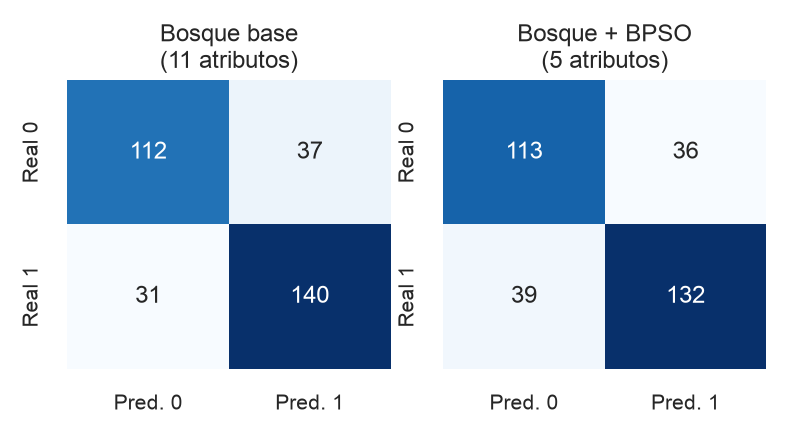
\includegraphics[width=\columnwidth]{figuras/matrices_confusion.png}
\caption{Matrices de confusión en prueba. Izquierda: once atributos. Derecha: cinco atributos seleccionados.}
\label{fig:cm}
\end{figure}

Durante la trayectoria de la semilla 42 apareció una máscara de ocho atributos con F1-macro de validación 0,789, superior al de la solución elegida. Su costo fue 0,248, peor que 0,236, por la penalización de tamaño. El criterio hizo lo que se le pidió: prefirió parsimonia frente a una ganancia de F1 inferior al precio de tres atributos adicionales. Esa máscara no se promovió a la prueba, porque la regla de selección estaba fijada de antemano.

\subsection{Atributos seleccionados}
La Fig.~\ref{fig:freq} resume la frecuencia de cada variable en la mejor máscara de cada semilla. Sulfatos y alcohol aparecen en las cinco. El azúcar residual y el dióxido de azufre total aparecen en cuatro. La acidez fija aparece en tres. El resto queda en dos apariciones o en una.

\begin{figure}[!t]
\centering
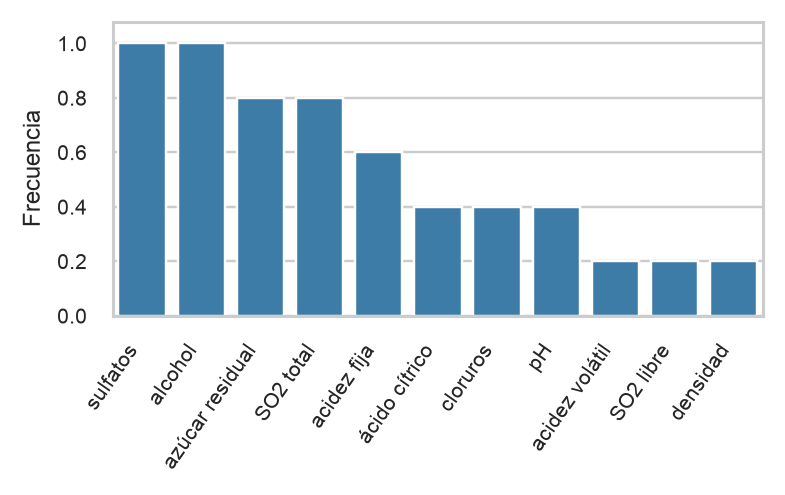
\includegraphics[width=\columnwidth]{figuras/frecuencia_atributos.png}
\caption{Frecuencia con la que cada atributo integra la mejor máscara de cada una de las cinco semillas.}
\label{fig:freq}
\end{figure}

La coincidencia de alcohol y sulfatos con las correlaciones de Spearman más informativas es plausible, pero no autoriza una lectura causal. El azúcar residual tiene correlación marginal casi nula y, sin embargo, entra en cuatro de cinco soluciones, incluida la ganadora. La acidez volátil, segunda asociación más fuerte con la puntuación, solo entra en una mejor máscara. El \emph{wrapper} está respondiendo a interacciones dentro del bosque, no al orden univariado. Con cinco semillas no corresponde declarar un subconjunto fisicoquímico estable ni recomendar el control de proceso de esas cinco variables.

\subsection{Convergencia}
La Fig.~\ref{fig:conv} corresponde a una sola trayectoria, la de la semilla seleccionada. Los puntos de las evaluaciones 10, 20 y 30 pertenecen a esa curva y no a experimentos separados. El mejor costo acumulado es 0,236 en los tres cortes. El costo de la partícula evaluada en esos instantes es peor: 0,248, 0,254 y 0,277. El incumbente se alcanzó en la evaluación 1 y no volvió a actualizarse. De las 30 llamadas, 18 fueron subconjuntos distintos; el resto reutilizó un costo ya calculado.

\begin{figure}[!t]
\centering
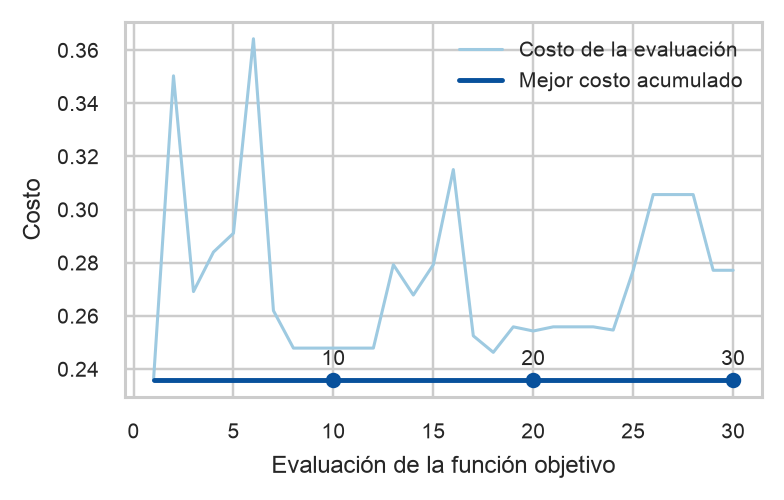
\includegraphics[width=\columnwidth]{figuras/convergencia_semilla_42.png}
\caption{Costo por evaluación y mejor costo acumulado en la semilla 42. El incumbente no cambia entre las evaluaciones 10, 20 y 30.}
\label{fig:conv}
\end{figure}

Las otras semillas sí actualizan el incumbente, aunque ninguna supera el costo inicial de la semilla 42. La semilla 7 mejora una vez y fija su mejor valor en la evaluación 13. La semilla 2024 lo hace en la evaluación 3. Las semillas 123 y 99 mejoran tres veces y alcanzan su mejor costo en las evaluaciones 19 y 26. Hay, por tanto, búsqueda efectiva en parte de las réplicas, pero la solución que el protocolo declara ganadora no es producto de esa mejora: es la primera partícula de la semilla más favorable. Con 30 evaluaciones se inspecciona alrededor del 1,5\,\% del espacio por ejecución, y las repeticiones reducen aún más los subconjuntos distintos. El estancamiento de la mejor trayectoria es una propiedad del presupuesto, no un detalle del gráfico.

\subsection{Estabilidad}
La Tabla~\ref{tab:runs} recoge la mejor solución de cada semilla. El costo medio es $0{,}247 \pm 0{,}007$, el F1-macro medio es $0{,}781 \pm 0{,}007$ y el número de atributos es $6{,}0 \pm 1{,}4$. El F1 de validación se mueve en un intervalo estrecho, por debajo o al nivel del baseline. El tamaño de la máscara no: oscila entre cinco y ocho atributos.

\begin{table*}[!t]
\caption{Mejor solución de cada ejecución independiente, medida en validación}
\label{tab:runs}
\centering
\footnotesize
\begin{tabular}{@{}rrrrlp{7.4cm}@{}}
\toprule
Semilla & Costo & F1-macro & $n$ & Tiempo (s) & Atributos retenidos \\
\midrule
42 & 0,236 & 0,787 & 5 & 5,59 & azúcar residual, SO$_2$ total, pH, sulfatos, alcohol \\
7 & 0,251 & 0,785 & 8 & 4,29 & acidez fija, ácido cítrico, azúcar residual, cloruros, SO$_2$ libre, SO$_2$ total, sulfatos, alcohol \\
123 & 0,247 & 0,776 & 5 & 5,88 & acidez fija, azúcar residual, SO$_2$ total, sulfatos, alcohol \\
2024 & 0,252 & 0,771 & 5 & 6,34 & acidez fija, azúcar residual, densidad, sulfatos, alcohol \\
99 & 0,248 & 0,784 & 7 & 6,52 & acidez volátil, ácido cítrico, cloruros, SO$_2$ total, pH, sulfatos, alcohol \\
\bottomrule
\end{tabular}
\end{table*}

El índice de Jaccard medio entre los diez pares de máscaras es 0,481. La intersección estable se reduce, en la práctica, a sulfatos y alcohol. El subconjunto ganador no puede presentarse como una selección reproducible del enjambre. Reportar solo la semilla 42 ocultaría esa dispersión.

\subsection{Costo computacional}
Las cinco búsquedas suman 28,63\,s. Cada una realiza 30 evaluaciones y entre 14 y 21 entrenamientos efectivos. En total hay 150 evaluaciones, 92 entrenamientos de la función objetivo y 58 aciertos de caché. Como cada entrenamiento efectivo repite tres ajustes de validación, el experimento realiza 276 ajustes de bosque durante la búsqueda, además del baseline y de los dos ajustes finales. El tiempo medio por evaluación, contando las repeticiones, queda entre 0,14 y 0,22\,s según la semilla.

El ajuste final del modelo reducido no es más rápido que el del modelo completo: 0,076\,s en ambos casos, dentro de la variación de una corrida corta. La evaluación en prueba tampoco cambia de orden (0,014\,s frente a 0,013\,s). El ahorro de variables no devuelve el tiempo invertido en la búsqueda. El costo de BPSO solo se justificaría por parsimonia o por una ganancia predictiva. La primera se obtiene; la segunda, en prueba, no.

\subsection{Lectura crítica}
BPSO no mejoró el modelo predictivo. La ligera ventaja de validación desaparece en la prueba y cambia de signo. La reducción de atributos sí es material, de once a cinco en la solución elegida, pero los subconjuntos de las otras semillas no confirman esa misma máscara. La estabilidad es baja más allá de alcohol y sulfatos. El costo de la búsqueda es pequeño en tiempo absoluto ---menos de medio minuto en la máquina utilizada--- y, aun así, no compra mejor generalización ni un ajuste final más barato.

Tres limitaciones condicionan cualquier generalización. Primera, el presupuesto cubre una fracción pequeña del espacio y la solución declarada ganadora no fue mejorada por el enjambre. Segunda, la misma validación que puntúa a las partículas sirve para elegir la semilla, de modo que el F1 de validación del ganador está expuesto a una selección optimista; la caída en prueba es consistente con ese riesgo. Tercera, hay una sola partición entrenamiento-prueba, la etiqueta aplana una escala ordinal y los tiempos dependen del paralelismo de la CPU. Los duplicados y los extremos se conservaron a propósito; otra decisión de limpieza podría mover las métricas, pero no fue parte del protocolo.

\section{Conclusiones}
Se comparó un Random Forest con las once variables fisicoquímicas de los vinos tintos de Wine Quality frente al mismo bosque restringido por un enjambre binario. El protocolo separó la prueba antes de la búsqueda, usó F1-macro con validación estratificada de tres particiones y fijó 30 evaluaciones por semilla en cinco réplicas.

El subconjunto elegido conserva cinco atributos y obtiene en validación un F1-macro de 0,787, indistinguible en la práctica del 0,783 del modelo completo. En prueba, el F1-macro baja de 0,786 a 0,764 y el AUC-ROC de 0,858 a 0,847. La reducción es grande; la mejora predictiva no aparece. Alcohol y sulfatos se seleccionan en todas las semillas, pero el Jaccard medio de 0,481 muestra que el resto de la máscara no es estable. La trayectoria ganadora alcanza su costo en la primera evaluación y permanece detenida en los cortes 10, 20 y 30. Las cinco búsquedas cuestan 28,63\,s y 276 ajustes de validación, sin reducir el tiempo del modelo final.

El experimento cumple el objetivo de cuantificar el compromiso entre atributos y desempeño. No sostiene reemplazar al modelo de once variables cuando la prioridad es la predicción en datos no usados. Una continuación útil, todavía dentro de este conjunto, sería contrastar el enjambre con la búsqueda exhaustiva de los 2048 subconjuntos, ampliar el presupuesto hasta observar mejoras posteriores a la inicialización y repetir la partición externa. Tratar \emph{quality} como variable ordinal, o ajustar el bosque solo después de haber fijado la máscara, respondería preguntas distintas de la que este trabajo dejó medida.

\begin{thebibliography}{12}

\bibitem{cortez2009}
P.~Cortez, A.~Cerdeira, F.~Almeida, T.~Matos, and J.~Reis, ``Modeling wine preferences by data mining from physicochemical properties,'' \emph{Decision Support Systems}, vol.~47, no.~4, pp.~547--553, 2009, doi: 10.1016/j.dss.2009.05.016.

\bibitem{uci186}
UCI Machine Learning Repository, ``Wine Quality,'' dataset no.~186. [Online]. Available: \url{https://archive.ics.uci.edu/dataset/186/wine+quality}

\bibitem{breiman2001}
L.~Breiman, ``Random forests,'' \emph{Machine Learning}, vol.~45, no.~1, pp.~5--32, 2001, doi: 10.1023/A:1010933404324.

\bibitem{kennedy1995}
J.~Kennedy and R.~Eberhart, ``Particle swarm optimization,'' in \emph{Proc. IEEE Int. Conf. Neural Networks (ICNN)}, vol.~4, 1995, pp.~1942--1948, doi: 10.1109/ICNN.1995.488968.

\bibitem{kennedy1997}
J.~Kennedy and R.~C. Eberhart, ``A discrete binary version of the particle swarm algorithm,'' in \emph{Proc. IEEE Int. Conf. Systems, Man, and Cybernetics}, vol.~5, 1997, pp.~4104--4108, doi: 10.1109/ICSMC.1997.637339.

\bibitem{guyon2003}
I.~Guyon and A.~Elisseeff, ``An introduction to variable and feature selection,'' \emph{J. Mach. Learn. Res.}, vol.~3, pp.~1157--1182, 2003.

\bibitem{kohavi1997}
R.~Kohavi and G.~H. John, ``Wrappers for feature subset selection,'' \emph{Artificial Intelligence}, vol.~97, no.~1--2, pp.~273--324, 1997, doi: 10.1016/S0004-3702(97)00043-X.

\bibitem{xue2013}
B.~Xue, M.~Zhang, and W.~N. Browne, ``Particle swarm optimization for feature selection in classification: A multi-objective approach,'' \emph{IEEE Trans. Cybern.}, vol.~43, no.~6, pp.~1656--1671, 2013, doi: 10.1109/TSMCB.2012.2227469.

\bibitem{xue2016}
B.~Xue, M.~Zhang, W.~N. Browne, and X.~Yao, ``A survey on evolutionary computation approaches to feature selection,'' \emph{IEEE Trans. Evol. Comput.}, vol.~20, no.~4, pp.~606--626, 2016, doi: 10.1109/TEVC.2015.2504420.

\bibitem{kohavi1995}
R.~Kohavi, ``A study of cross-validation and bootstrap for accuracy estimation and model selection,'' in \emph{Proc. 14th Int. Joint Conf. Artificial Intelligence (IJCAI)}, 1995, pp.~1137--1143.

\bibitem{miranda2018}
L.~J.~V. Miranda, ``PySwarms: a research toolkit for particle swarm optimization in Python,'' \emph{J. Open Source Softw.}, vol.~3, no.~21, p.~433, 2018, doi: 10.21105/joss.00433.

\bibitem{pedregosa2011}
F.~Pedregosa \emph{et al.}, ``Scikit-learn: Machine learning in Python,'' \emph{J. Mach. Learn. Res.}, vol.~12, pp.~2825--2830, 2011.

\end{thebibliography}

\end{document}
